
\begin{center}
	\Huge
	Middelværdi og spredning fra stikprøve
\end{center}
\section*{Estimation af parametre}
\stepcounter{section}

I de eksempler, vi har arbejdet med, har vi antaget, at middelværdien og spredningen er kendte værdier, men dette vil kun meget sjældent være tilfældet i normalfordelte stokastiske variable, der beskriver virkelige fænomener. Vi skal derfor have en måde at estimere middelværdien $\mu$ og spredningen $\sigma$ for den underliggende normalfordelte stokastiske variabel $X$, vi forventer kan beskrive vores stikprøve. Middelværdien for en stokastisk variabel er et slags ikke-realiseret gennemsnit, og derfor estimerer vi den ved at bestemme gennemsnittet af datasættet. 

\begin{defn}[Gennemsnit og spredning]
Lad $x_1,x_2,\hdots, x_n$ være en stikprøve. Så defineres middelværdiestimatet $\hat{\mu}$ som gennemsnittet af stikprøven
\begin{align*}
	\hat{\mu} = \frac{x_1+x_2+\cdots+x_n}{n}.
\end{align*}
Spredningsestimatet $\hat{\sigma}$ defineres som kvadratroden af den gennemsnitlige kvadratiske variation fra middelværdien
\begin{align*}
	\hat{\sigma} = \sqrt{\frac{(x_1-\hat{\mu})^2 + (x_2 - \hat{\mu})^2+\cdots + (x_n-\hat{\mu})^2}{n}}. 
\end{align*}
Til tider bruges også spredningsestimatet $s$ givet ved
\begin{align*}
	s = \sqrt{\frac{\sum_{i=1}^n\left({x_i - \hat{\mu}}\right)^2}{n-1}}.
\end{align*}
\end{defn}
Dette er i princippet et bedre bud på den \textit{rigtige} spredning, men vi vil ikke komme præcist ind på hvorfor. Intuitionen er dog følgende; stikprøveværdierne $x_i$ ligger generelt tættere på stikprøvemiddelværdien $\hat{\mu}$ end på den rigtige middelværdi $\mu$, og derfor vil spredningen blive lidt for lille. Ved at betragte den gennemsnitlige afstand mellem $\hat{\mu}$ og $\mu$ kan man så komme frem til estimatet $s$. 
\begin{exa}
Vi har følgende \href{https://github.com/ChristianJLex/TeachingNotes/raw/master/2022-2023/Data%20og%20lign/data.xlsx}{\color{blue!60}data}, og vi ønsker at bestemme middelværdien og spredningen for datasættet. Dette gøres i Maple ved at skrive
\begin{align*}
	&\texttt{with(Gym):}\\
	&\texttt{middel(Data)}\\
	&\texttt{spredning(Data)}
\end{align*} 
Vi gør dette i Maple og får, at middelværdien er
\begin{align*}
	\hat{\mu} = 198.97
\end{align*}
og spredningen er 
\begin{align*}
	\hat{\sigma} = 15.19.
\end{align*}
\end{exa}

\section*{Er data normalfordelt?}
\stepcounter{section}

Vi vil gerne kunne afgøre, om et datasæt er normalfordelt. Til dette laver vi det, vi kalder et \textit{fraktilplot}. Først skal vi dog bruge en sætning, der siger noget om, hvordan vi transformerer en normalfordelt stokastisk variabel til en standardnormalfordelt stokastisk variabel. 

\begin{setn}
	Lad $X \sim N(\mu, \sigma)$ være en normalfordelt stokastisk variabel og lad
	\begin{align*}
		Z = \frac{X-\mu}{\sigma}.
	\end{align*}
	Så gælder der, at 
	\begin{align*}
		Z \sim N(0,1).
	\end{align*}
\end{setn}
\begin{proof}
	Vi betragter fordelingsfunktionen for $Z$:
	\begin{align*}
		P(Z<a) &= P(\frac{X-\mu}{\sigma} \leq a)\\
		&= P(X-\mu < a\sigma)\\
		&= P(X < a\sigma+\mu)\\
		&= \int_{-\infty}^{a\sigma+\mu}\frac{1}{\sigma\sqrt{2\pi}}e^{-\frac{1}{2}\left(\frac{x-\mu}{\sigma}\right)^2}dx.
	\end{align*}
	Vi laver nu substitutionen 
	\begin{align*}
		z = \frac{x-\mu}{\sigma},
	\end{align*}
	og får, at
	\begin{align*}
		\frac{dz}{dx} = \frac{x}{\sigma}
	\end{align*}
	og dermed, at 
	\begin{align*}
		dz\sigma = dx.
	\end{align*}
	For at lave substitutionen skal vi tilsvarende ændre grænserne. Den nedre grænse giver
	\begin{align*}
		\frac{-\infty - \mu}{\sigma} = -\infty,
	\end{align*}
	og den øvre grænse giver
	\begin{align*}
		\frac{a\sigma+\mu -\mu}{\sigma} = a.
	\end{align*}
	Vi substituerer
	\begin{align*}
		\int_{-\infty}^{a\sigma+\mu}\frac{1}{\sigma\sqrt{2\pi}}e^{-\frac{1}{2}\left(\frac{x-\mu}{\sigma}\right)^2}dx &= 
		\int_{-\infty}^a\frac{1}{\sigma\sqrt{2\pi}}e^{-\frac{1}{2}z^2}dz\sigma\\
		&=\int_{-\infty}^a\frac{1}{\sqrt{2\pi}}e^{-\frac{1}{2}z^2}dz\\
		&= \int_{-\infty}^a\varphi(z)dz \\
		&= \Phi(a).
	\end{align*}
	Da $Z$ har $\Phi$ som fordelingsfunktion, så må $Z$ være standardnormalfordelt. 
\end{proof}

Vi ved, at $\Phi$ er en voksende funktion. Den har derfor en invers funktion $\Phi^{-1}$. Da $X \sim N(\mu,\sigma)$ har fordelingsfunktion
\begin{align*}
	F(x) = \Phi\left(\frac{x-\mu}{\sigma}\right),
\end{align*} 
så må der gælde, at 
\begin{align*}
	z = \Phi^{-1}(F(x)) = \Phi^{-1}\left(\Phi\left(\frac{x-\mu}{\sigma}\right) \right) = \frac{x-\mu}{\sigma}.
\end{align*}
Vi kan altså teste om et datasæt er normalfordelt ved at plotte dataet op mod de teoretiske $z$-værdier. Følger disse den rette linje
\begin{align*}
	z = \frac{x-\mu}{\sigma},
\end{align*}
så vil datasættet forventes at være normalfordelt. Dette er intuitionen bag fraktilplottet. Det laves i Maple ved at skrive
\begin{align*}
	&\texttt{with(Gym):}\\
	&\texttt{QQplot(Data)}
\end{align*}
\begin{exa}
	Vi har lavet et fraktilplot på datasættet fra før i Maple. Dette kan ses af Fig. \ref{fig:QQ}.
	\begin{figure}[H]
		\centering
		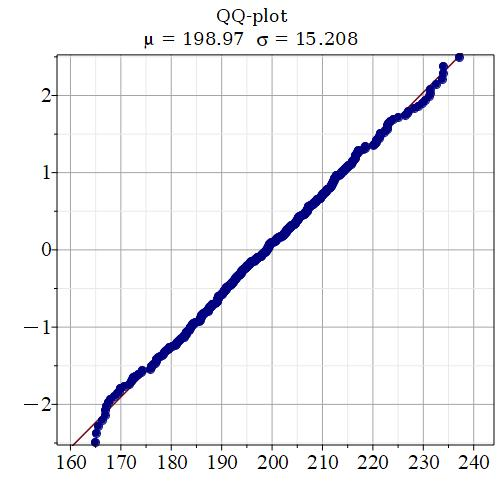
\includegraphics[width=0.7\textwidth]{Billeder/QQ.jpg}
		\caption{Fraktilplot for datasæt}
		\label{fig:QQ}
	\end{figure}
	Dataet ligger pænt langs med den rette linje $z = (x-198.97)/15.208$, og vi antager derfor, at det er normalfordelt. 
\end{exa}


\section*{Opgave 1}
\href{https://github.com/ChristianJLex/TeachingNotes/raw/master/2022-2023/Data%20og%20lign/IQdata.xlsx}{\color{blue!60}Dette data} beskriver IQ for 213 værnepligtige. 
\begin{enumerate}[label=\roman*)]
	\item Bestem middelværdi og spredning for IQ af de værnepligtige.
	\item Afgør, om dataen kan antages at være normalfordelt. 
	\item Bestem sandsynligheden for at have en IQ på under 130.
	\item Bestem det tal, så 99$\%$ af befolkningen har en IQ på mindre end $x$. 
\end{enumerate}

\section*{Opgave 2}
173 raske personer har fået målt deres temperatur. Resultatet er i \href{https://github.com/ChristianJLex/TeachingNotes/raw/master/2022-2023/Data%20og%20lign/Temperaturdata.xlsx}{\color{blue!60} dette datasæt}.
\begin{enumerate}[label=\roman*)]
	\item Bestem middelværdi og spredning for temperaturen.
	\item Afgør, om dataen kan antages at være normalfordelt. 
	\item Bestem sandsynligheden for at have en temperatur på under 40 grader. 
	\item Bestem sandsynligheden for at have en temperatur mellem 35 og 38 grader.  
\end{enumerate}


\section*{Opgave 3}
501 kvinder har målt deres højde. Resultatet kan findes \href{https://github.com/ChristianJLex/TeachingNotes/raw/master/2022-2023/Data%20og%20lign/Hojdedata.xlsx}{\color{blue!60}her}.
\begin{enumerate}
	\item Bestem middelværdi og spredning for højden.
	\item Afgør, om dataen kan antages at være normalfordelt.
	\item Bestem sandsynligheden for, at en kvinde er mindre end 150 cm
	\item Bestem et $95\%$-konfidensinterval for den rigtige middelværdi $\mu$. 
\end{enumerate}
